\chapter{Pithos Implementation}
\label{chp:IMPLEMENTATION}

The previous chapter discussed the conceptual design of Pithos. Pithos has been implemented in Oversim \cite{OverSim_2007}, a P2P simulation environment based in Omnet++ \cite{omnetpp}, which allows for the measurement of identified requirements. Furthermore, it allows for the comparison of the current model with other state persistency models available in Oversim.

\section{Oversim}

Oversim is a peer-to-peer and overlay simulation framework for the Omnet++ simulator. Oversim allows for the simulation of many well known structured or unstructured overlay protocols. It also allows for the development of applications that can use the already implemented overlays in a well defined architecture.

\subsection{Motivation}

To allow for greater control of the environment, as well as greater scale, it was decided to implement the first version of Pithos as a large scale network simulation. A simulation allows for careful selection of the environment parameters and precise control of the parameter values. This in turns allows one to keep all but one parameter constant and evaluate the effect of a design decision on the system for varying values of the free parameter.

The underlying Omnet++ simulation environment is a powerful network simulator in its own right. It allows for robust message and module definitions and contains many tools to assist with simulation measurement and monitoring, for example global statistics gathering tools and built-in plotting tools.

Simulation also allows for greater scalability and simulating on a network with global Internet characteristics. Greater scalability is achieved, because thousands of nodes can easily be created, where all the nodes have global scale latency characteristics.

Implementing a large scale network application in the real-world would require thousands of computers spread across the globe. Such an environment will contain many variables out of the designer's control. For example, issues such as router congestion vary from day to day, which will produce varying latency results.

Because of these reasons, it was decided to first implement Pithos in simulation. This allows for the perfection of the design, under laboratory conditions, before the real world implementation is completed.

Pithos is intended for future real world implementation, however, so all modules created were written in such a manner to allow for easy porting. No tasks that are performed in Pithos make use of any simulation ``short cuts'', such as accessing the global peer list. Only statistics gathering modules are allowed to make use of these simulation features.

\subsection{Underlay network}
\label{oversim_underlay}

At the base of an Oversim simulation is the underlay network. The underlay network determines the types of nodes in the Oversim simulation. Three underlay types exist: the ``simple'', ``INET'' and ``SingleHost'' underlays \cite{oversim_applications}.

A node type is determined by the protocols executing on every layer of the Oversim architecture. As discussed in Section \ref{key_modules_mechs}, the Pithos node types are the peer, super peer and directory server.

For the Pithos simulation, reliable communication was assumed. It was also assumed that nodes have sufficiently large receive buffers to buffer all required messages until they are handled. No message ordering was assumed. Messages are allowed to be received in a different order than the order they were sent in. This, in fact, always happens when a larger message is sent before a smaller message.

The time that a message is scheduled to be received at the destination is the time when the message would have been fully received by the destination.

\subsubsection{Latency profiles}
In the simple underlay, node latencies are determined by the distance between nodes placed in a two dimensional Euclidean space. The positions of the nodes are chosen to match the latencies of the CAIDA/Skitter Internet mapping project \cite{caida_skitter}. Different nodes are also assigned different bandwidth and jitter parameters to simulate a heterogenous network. The simple underlay, therefore, captures the delay characteristics of a global scale network in an abstract way. The simple underlay network is ideal for simulating large scale overlay networks because of its simplicity and high accuracy \cite{oversim_applications}.

The INET underlay is based on the Omnet++ INET underlay and allows for the simulation of the complete IP level stack. This includes backbone routers and gateways. It also contains many implemented MAC layer protocols. The INET underlay is well suited to simulating lower level communication protocols or wireless protocols such as IEEE 802.11 (Wi-Fi).

The SingleHost underlay allows for interaction with a physical network. It allows for the implementation of physical nodes, running on networks computers. These physical nodes can then connect to a simulated network and receive packets with bandwidth and delay characteristics as if they were situated on a network with the simulation's specific characteristics.

\begin{figure}[htbp]
 \centering
 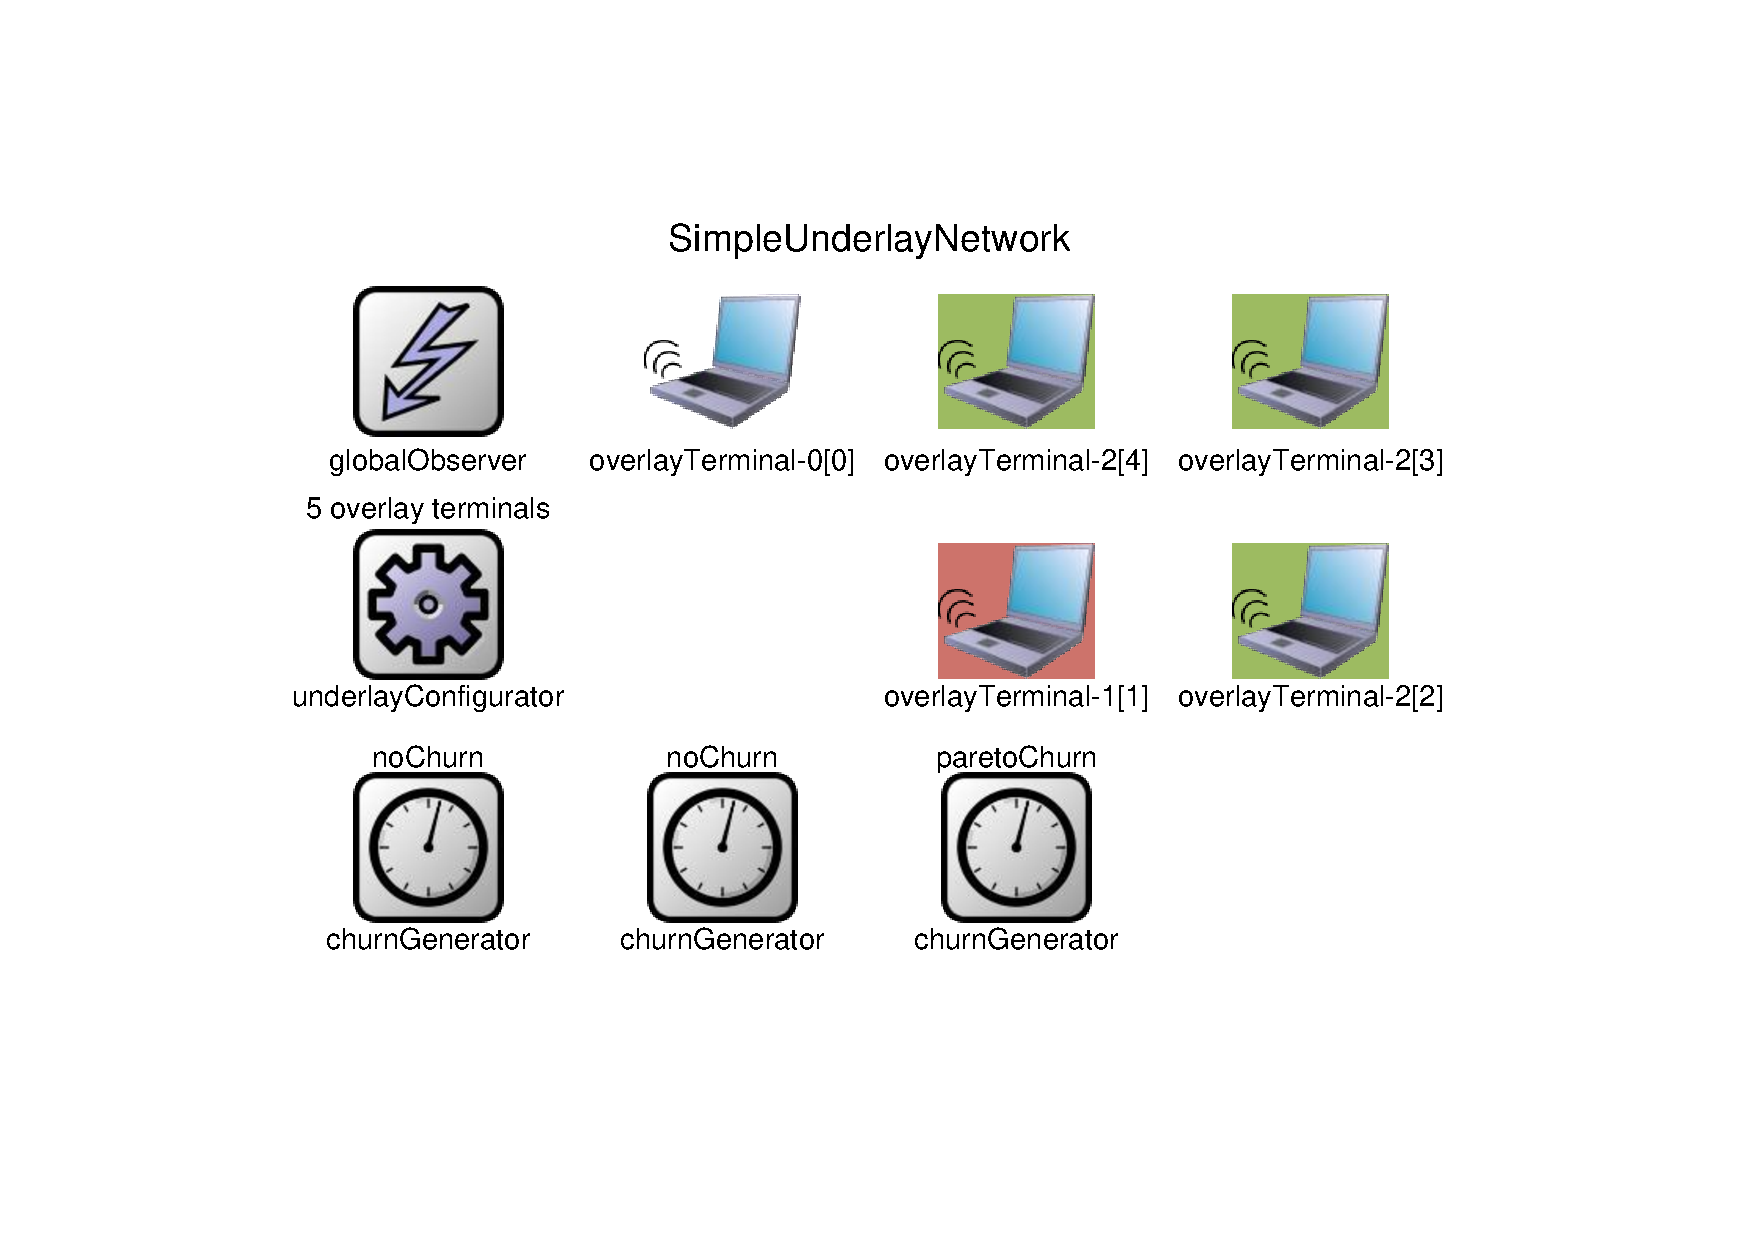
\includegraphics[clip=true, viewport=49mm 48mm 245mm 173mm, width=0.5\columnwidth]{Oversim_terminals}
 \caption{The Oversim simple underlay network with the three Pithos terminal types}
 \label{fig_oversim_terminals}
\end{figure}

Figure \ref{fig_oversim_terminals} shows the Pithos simple underlay network after the first five nodes have been generated. Each overlay terminal is an Oversim node containing its own protocol stack. The underlay configurator is responsible for setting up the network. The global observer contains the global node list, global statistics and parameters modules. It is used to generate global statistics and by the lower levels to keep track of all nodes.

\subsubsection{Churn generation}
Three churn generators also exist, one for generating each of the three Pithos node types. Churn generators model users joining and leaving the network. There are three types of churn generators: ``no churn'', ``lifetime churn'' and ``Pareto churn''. The ``no churn'' churn generator creates nodes every specified number of seconds until a specified number of nodes are reached and does nothing further. This generator can be used to test simple networks, where churn is not an issue, or for initial testing of the first prototype.

Lifetime churn creates nodes with specified average lifetimes, sampled from an exponential distribution. This is a distribution regularly used to model lifetimes in reliability engineering. Pareto churn samples node lifetimes from a Pareto distribution (type of heavy-tailed distribution), instead of an exponential distribution. Pareto churn requires mean node lifetime as well as mean node dead time to be specified.

\subsubsection{Exponential versus Pareto lifetime distributions}
\label{exp_vs_pareto}

\begin{figure}[htbp]
 \centering
 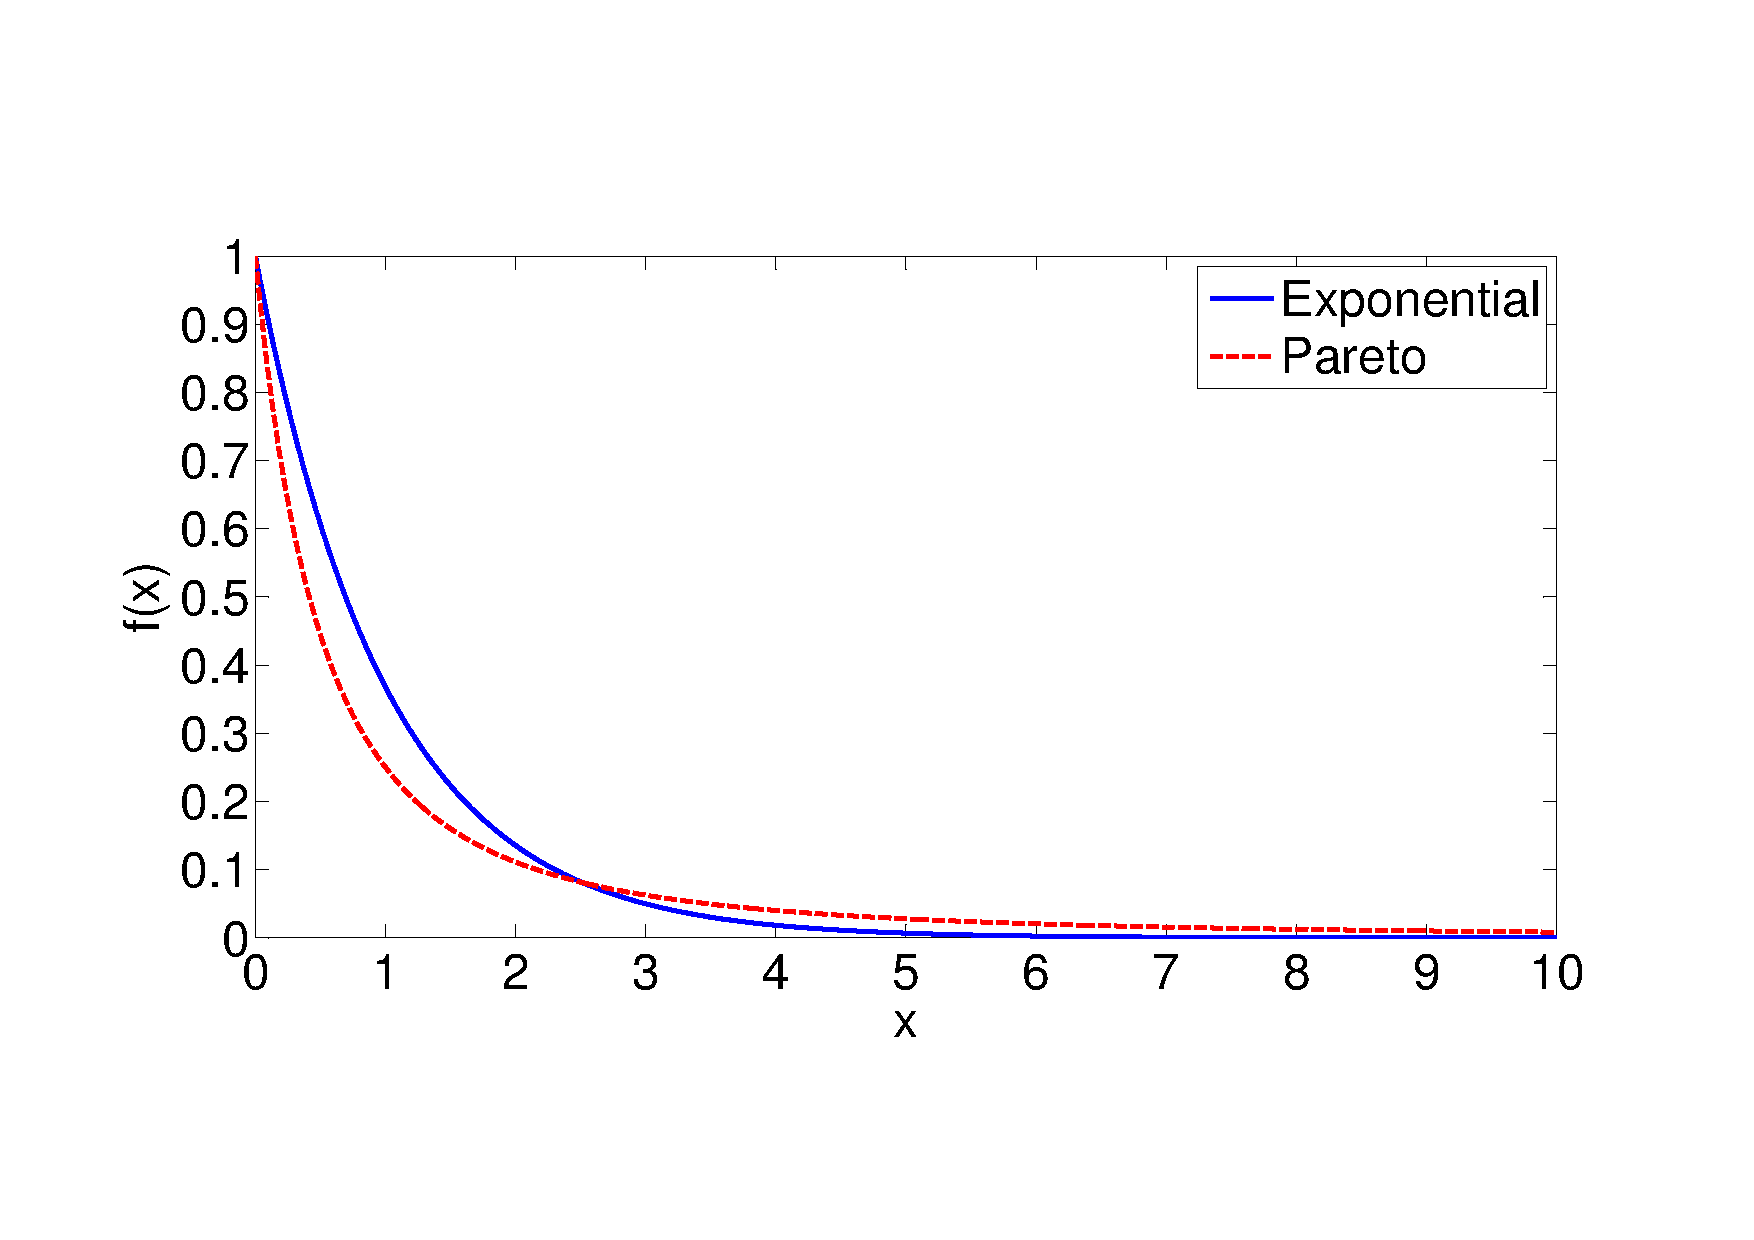
\includegraphics[clip=true, viewport=20mm 35mm 270mm 170mm, width=0.7\columnwidth]{exp_pareto_dist}
 \caption{Pareto distribution with shape parameter $K=1$ and scale parameter $\sigma=1$ and exponential distribution with rate parameter $\lambda=1$.}
 \label{fig_exp_pareto_dists}
\end{figure}
%
Figure \ref{fig_exp_pareto_dists} shows the probability density functions (PDFs) of the two types of lifetime distributions that are regularly used in reliability engineering: the exponential and the Pareto distribution \cite{rausand2004systemreliability}. The Pareto distribution has a shape similar to the exponential distribution, but with a heavy tail. For a shape parameter of $K=0$, the Pareto distribution is equivalent to the exponential distribution.

The advantage of the exponential distribution is its constant failure rate (hazard rate), which for node lifetimes is equivalent to a constant departure rate. The constant departure rate simplifies statistical models making use of the node failure rate parameter, as will be seen in Chapter \ref{chp:MODELLING}.

Even though the exponential lifetime distribution is simpler to work with, the Pareto distribution has been shown to more closely match user session times in online games \cite{Kwok_dist_match}. During the Pithos evaluation, the results from both distributions are compared. The disadvantage of the Pareto distribution is that its failure rate is a function of node lifetime.

\subsection{Node architecture}

\begin{figure}[htbp]
 \centering
 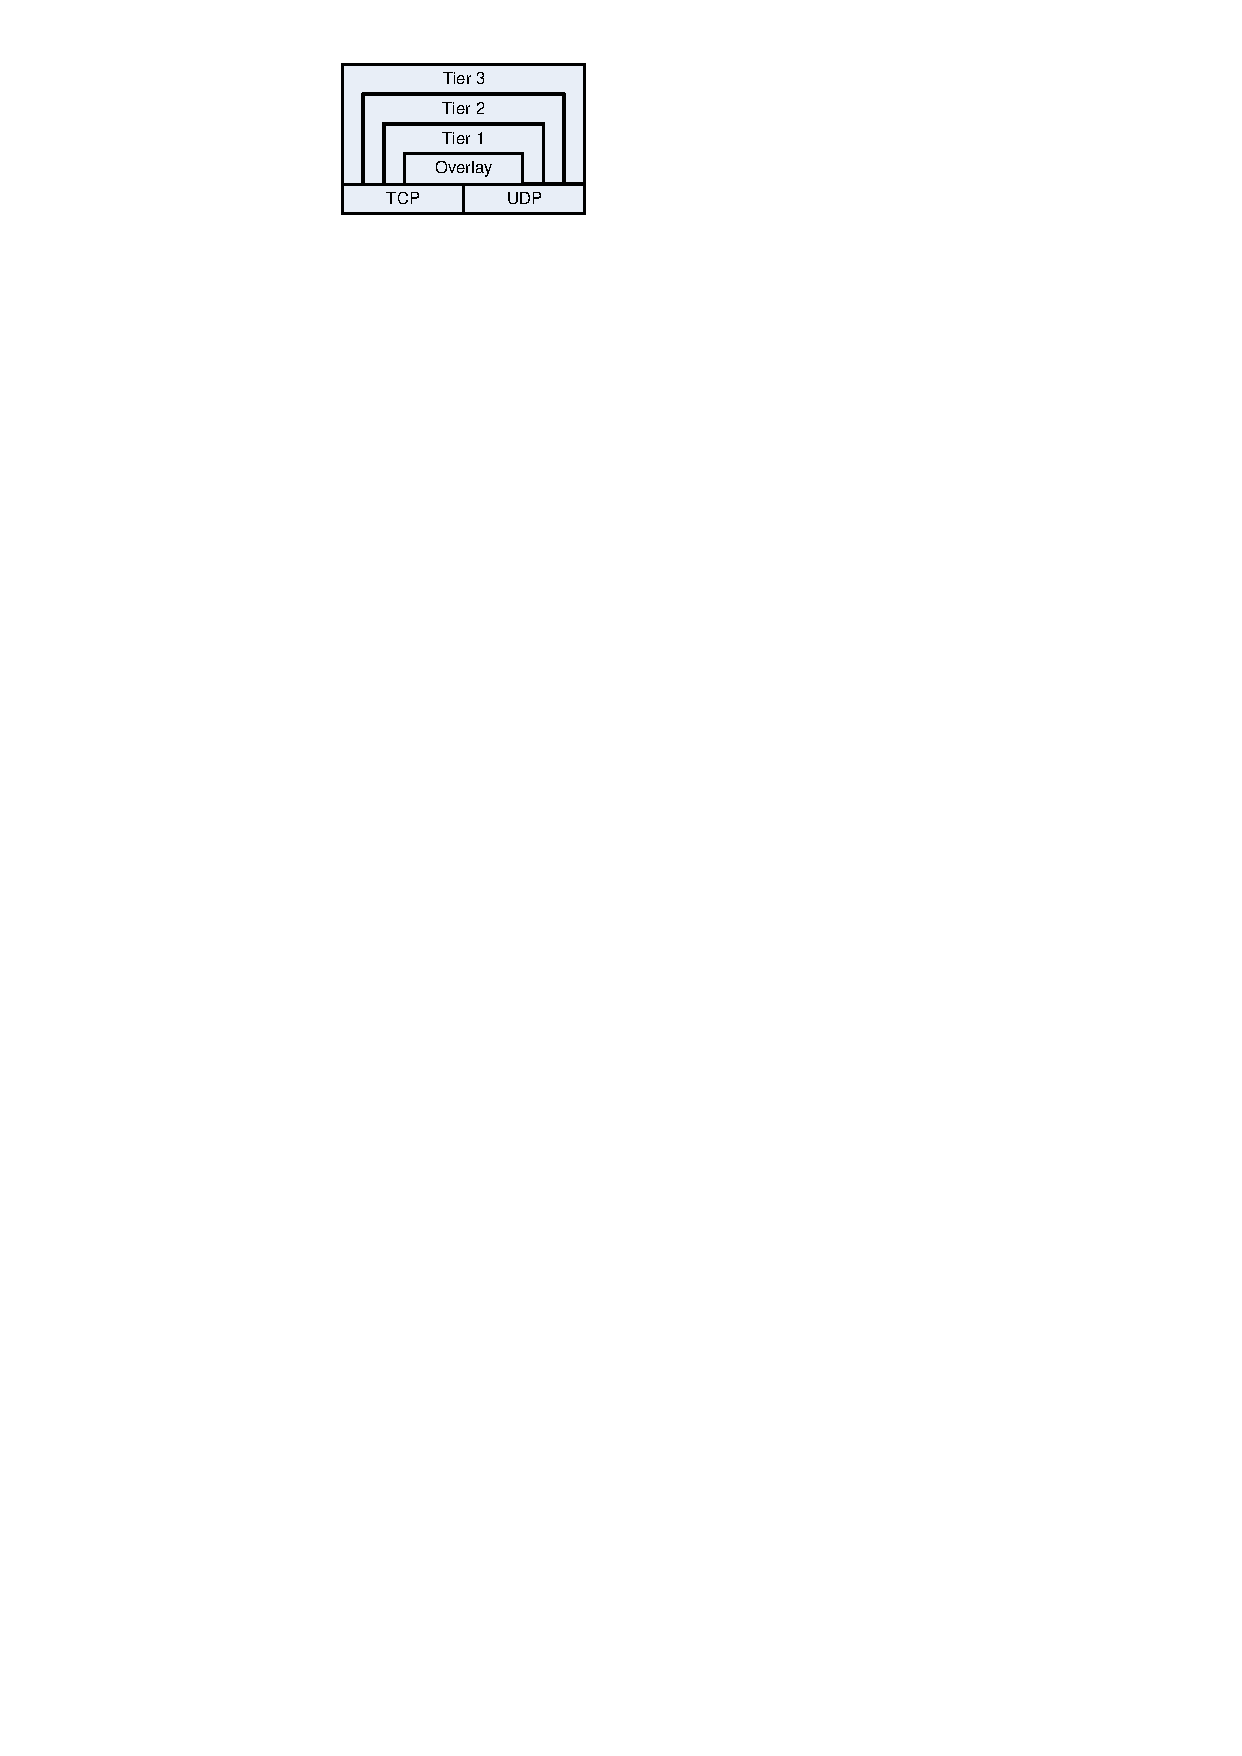
\includegraphics[clip=true, viewport=57mm 260mm 100mm 287mm, width=0.5\columnwidth]{Oversim_layers}
 \caption{Oversim node architecture layers}
 \label{fig_oversim_layers}
\end{figure}

%Also show the Oversim picture

Every node in Oversim contains a layered architecture, as shown in Figure \ref{fig_oversim_layers}. The Oversim node architecture contains the layers: TCP, UDP, Overlay, Tier 1, Tier 2 and Tier 3.

The transport control protocol (TCP) and user datagram protocol (UDP) are both transport level protocols, according to the OSI protocol stack specification. These two layers are the lowest communications layers in Oversim and allows message passing to other nodes.

The overlay layer is where the P2P overlay is housed. This can be any of the well known structured or unstructured overlays, such as Pastry, Chord or Gia \cite{Chawathe_gia}. The three tiers above the overlay layer are the application level layers and is where application that use an overlay may be implemented. Three application layers are allowed.

Tier 1 can communicate with the Tier 2, overlay, TCP and UDP layers. Tier 2 can communicate with the Tier 1, Tier 3, TCP and UDP layers. Tier 3 can communicate with the Tier 2, TCP and UDP layers. Internal communications are usually between tiers and TCP and UDP communication occurs when a layer wishes to send a message to the same layer on a different node.

\begin{figure}[htbp]
 \centering
 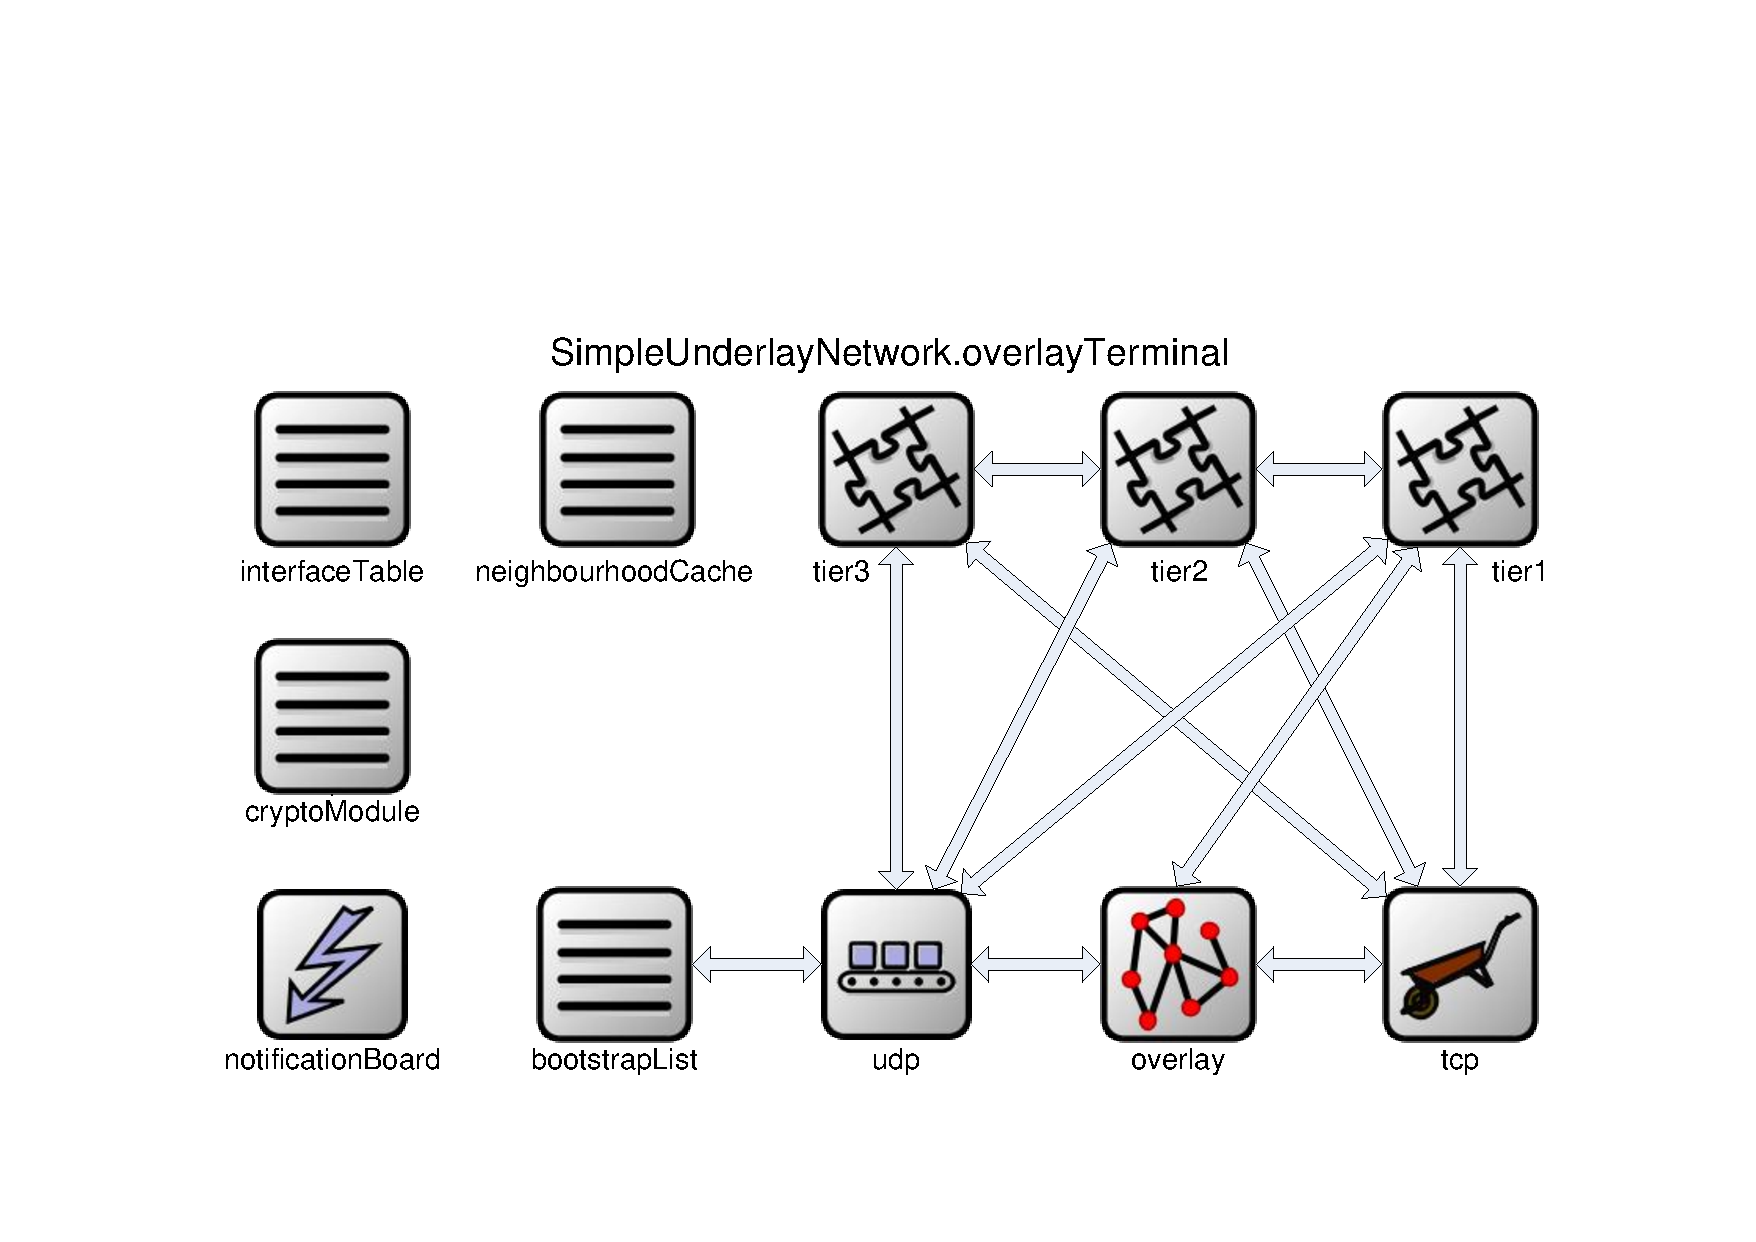
\includegraphics[clip=true, viewport=37mm 27mm 263mm 155mm, width=0.8\columnwidth]{Oversim_architecture}
 \caption{Components of an Oversim terminal, including the tiered node architecture.}
 \label{fig_oversim_architecture}
\end{figure}
%
Figure \ref{fig_oversim_architecture} shows the complete Oversim node architecture. The tiers, udp, tcp and overlay are connected as explained earlier. UDP is also connected to a bootstrap list module, which assists nodes with joining the UDP network. The neighbourhood cache, interface table, crypto module and notification board modules are also present, but these modules are unused in Pithos.

    \subsection{Generic consistency extension}
    \label{generic_consistency_extension}

To allow for the evaluation of Pithos as a module of a larger generic state consistency architecture, we extended the Oversim framework itself to simulate a complete request stream. The three tiers were replaced with all the elements identified in the generic consistency model in Section \ref{generic_event_update_model} for a single generic stream. Practically, this required the implementation of a new type of overlay terminal type, replacing the tiers with the layers shown in Figure \ref{fig_mmvehost_architecture}.
%
\begin{figure}[htbp]
 \centering
 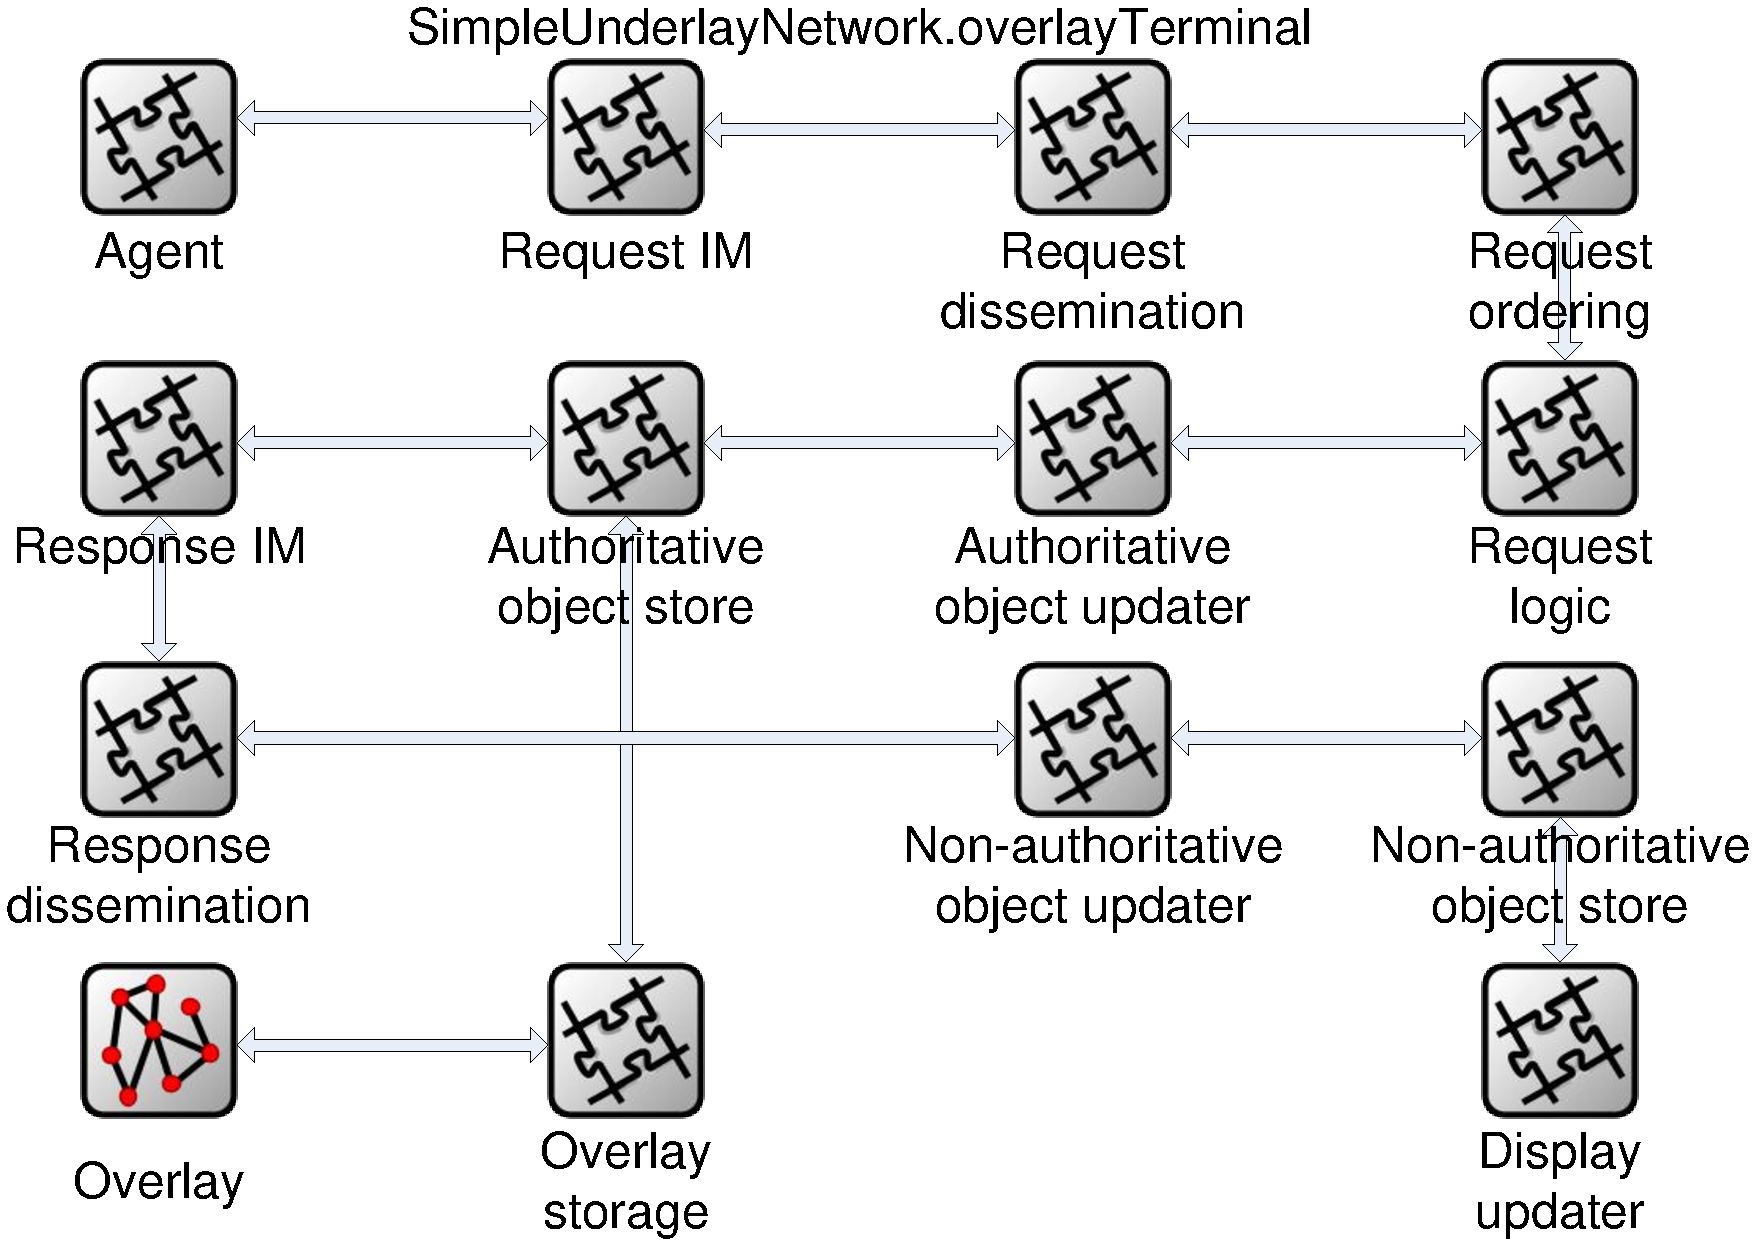
\includegraphics[width=0.8\columnwidth]{MMVEHost_architecture}
 \caption{Components of the expanded Oversim terminal, including all modules required for the generic consistency model.}
 \label{fig_mmvehost_architecture}
\end{figure}

Apart from the modules shown in Figure \ref{fig_mmvehost_architecture}, all other Oversim terminal modules that were shown in Figure \ref{fig_oversim_architecture} are still present (apart from the three tiers) and all of the modules shown in Figure \ref{fig_mmvehost_architecture} are also connected to the UDP and TCP modules, as with the tiers in the original Oversim module.

Every new layer can communicate with the layer above and below it, and can also communicate with its counterpart on another node using UDP or TCP. This allows for the consistency model to be distributed amongst any number of nodes. A module can either send its information to the layer below it within the same node, or it can send it to the layer below it on another node.

A difference between the generic model and the Oversim implementation is the two modules: ``overlay storage'' and ``overlay''. The ``overlay storage'' module houses the third-party overlay storage implementation and the implementation requires a separate overlay routing module. The separation is, therefore, for practical reasons. Conceptually, both the overlay storage and overlay modules form part of the authoritative object store.

Every module can contain a collection of sub-modules which implements the layer itself. If the layer is not implemented, a dummy layer is specified. The Pithos implementation is located within the authoritative object store module. An application that provides Pithos with test inputs called ``PithosTestApp'' is situated within the authoritative object updater layer. Pithos also makes use of overlay storage, which is implemented in the overlay storage module. Overlay storage requires a P2P overlay for routing purposes, which is why it is connected to the overlay layer.

\section{Module types}
\label{pithos_module_types}

\begin{figure}[htbp]
 \centering
 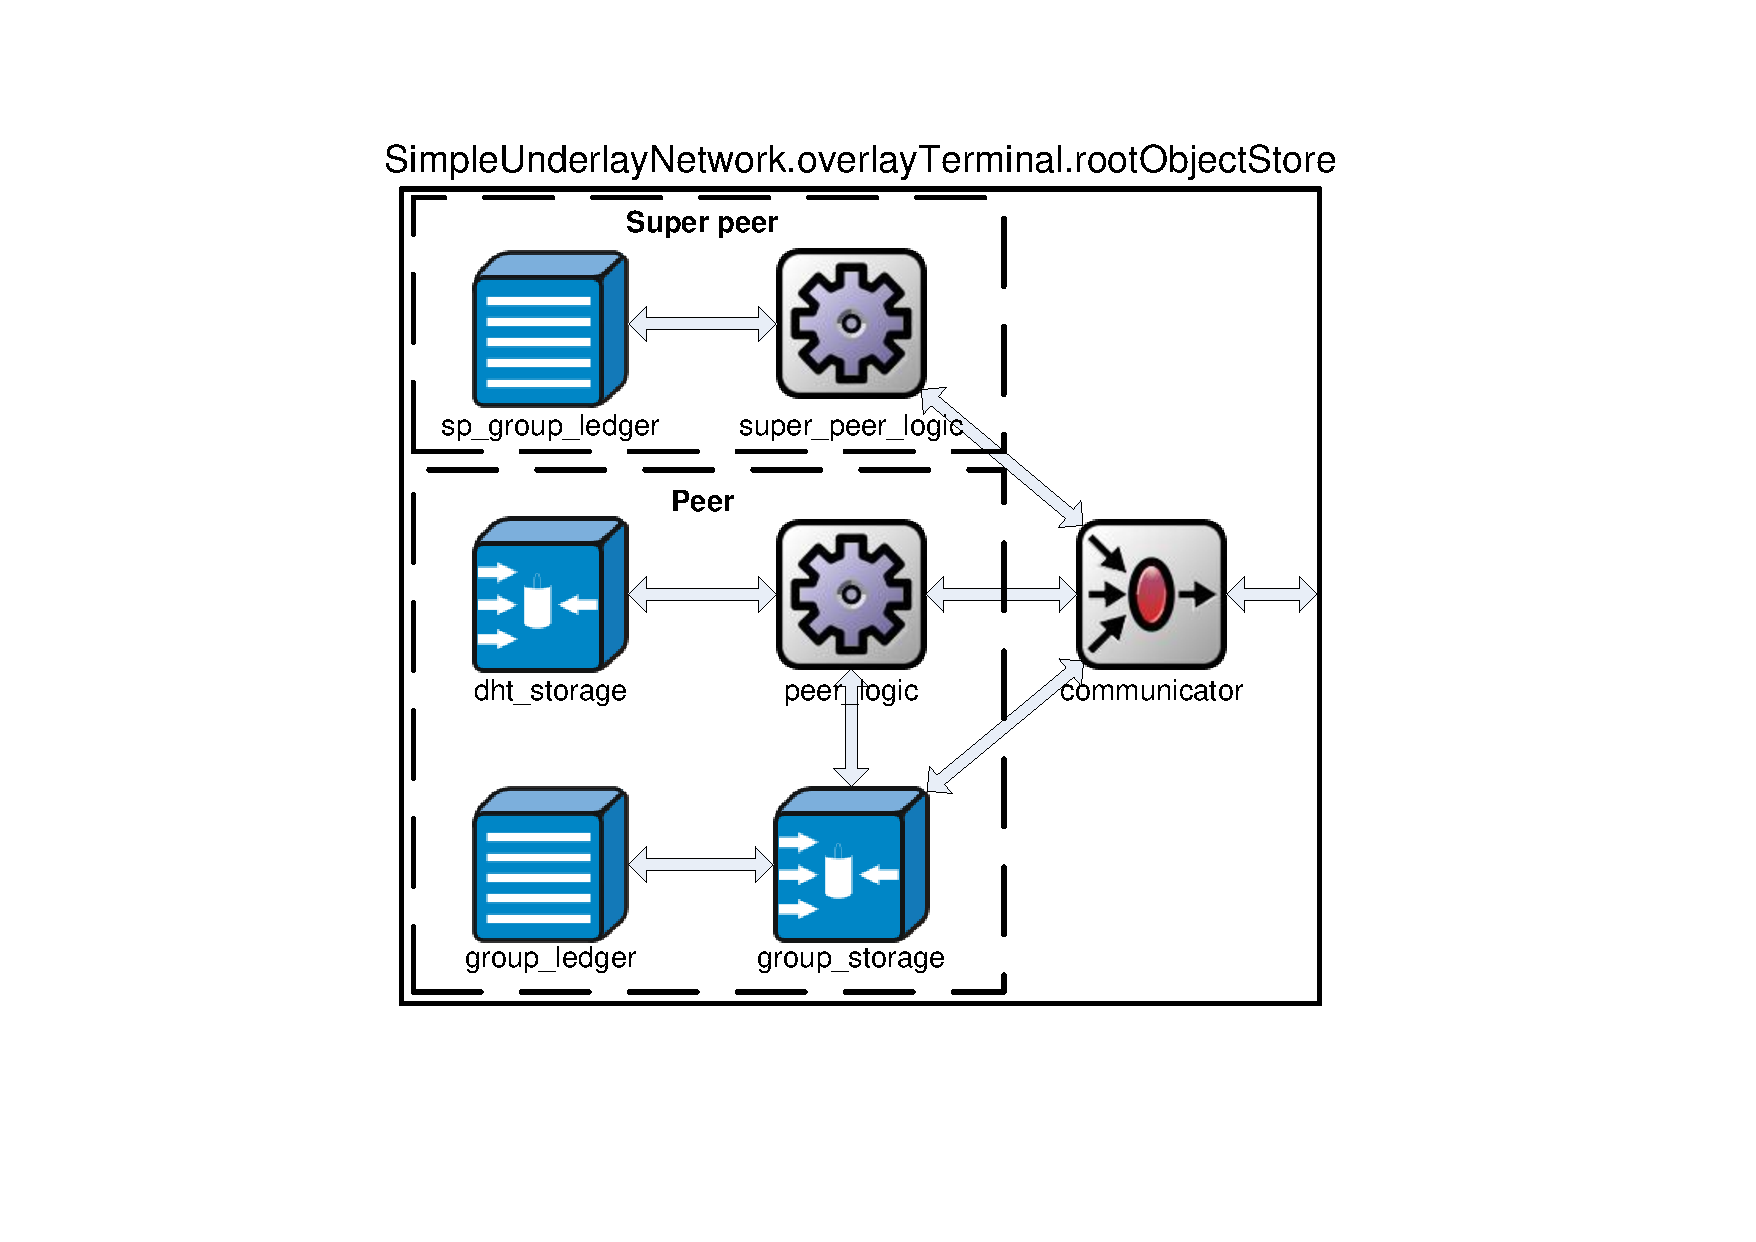
\includegraphics[clip=true, viewport=64mm 39mm 227mm 186mm, width=0.5\columnwidth]{Oversim_root_object_store}
 \caption{Pithos super peer and peer modules in Oversim}
 \label{fig_oversim_root_object_store}
\end{figure}
%
A simple module in Omnet++ is a module that implements a C++ class. All modules in Figure \ref{fig_oversim_root_object_store} are simple modules. Compound modules also exist that are combinations of simple modules, where the simple modules are connected to each other and external gates in some way.

Oversim requires a single simple module to be of type: ``BaseApp''. Oversim delivers messages from the layers above and below a layer to the module extending the BaseApp module. This means that because of Oversim's architecture, all messages must traverse a single module. When Pithos was designed, it was decided that placing all functionality in a single module would be a bad design decision, going against the philosophy of modular design. A single module would not allow for a modular implementation and would make future extensions more difficult.

Therefore, a communicator module was implemented to meet Oversim's requirement of all messages traversing a single module. The super peer and peer functionality is then implemented in seperate modules as shown in Figure \ref{fig_oversim_root_object_store}.

\subsection{Communicator}

The communicator module receives and sends all communications to the upper and lower layers on behalf of the other Pithos modules. All messages received or sent are, therefore, routed through the communicator module. The design philosophy of the communicator module was to make it as transparent as possible. Another function of the communicator module was outbound message verification. The communicator module ensures that all sent messages contain a destination IP address, source IP address and packet type information.

Transparency was achieved by designating certain gates for certain types of traffic. If a message is received on a gate with a specific purpose, that message is processed in a way consistent with that purpose and then transmitted. This design allows other modules to be expanded with new message types. Those message then only have to be sent to the correct gate to ensure correct handling of the message. The addition of a new message type, therefore, rarely required alterations to the communicator module.

\subsection{Peer node}

The peer module is responsible for group and overlay storage. It therefore requires a group ledger to keep track of objects in the group. It also needs access to the overlay storage and to implement local group storage. The group peer logic implements all the required group peer mechanisms, which include joining the group, leaving the group, repairing objects and handling store, retrieve and modify requests for the group.

\subsubsection{Peer logic}
Peer logic
\begin{enumerate}
  \item  receives all store, retrieve and modify requests from the higher application layer,
  \item forwards those requests to the required modules,
  \item forwards responses received from modules to the higher layer,
  \item keeps track of all outstanding requests (Section \ref{pending_rpcs_implementation}), and
  \item implements the quorum mechanism.
\end{enumerate}

\subsubsection{DHT storage}

The DHT storage module forms part of the peer node. The DHT storage module interfaces with the overlay storage module on behalf of the peer. The DHT storage module received requests from the peer logic modules for overlay storage services. The DHT storage module also keeps track of all outstanding overlay storage requests.

In the Oversim simulation, the DHT storage module interfaces with Oversim's DHT implementation, written by Gregoire Menuel and Ingmar Baumgart. The DHT implementation itself is located in the overlay storage module of the extended Oversim node architecture that represents the generic consistency model, as described in Section \ref{generic_consistency_extension}.

The Oversim DHT implementation contains data structures to store data, route requests via the overlay to other DHT modules and allows peers to join a network-wide overlay. It supports store, retrieve and modify requests. The Oversim DHT implementation meets all Pithos's overlay storage requirements and is able to run on any of the overlay implemented in Pithos.

\subsubsection{Group storage}

The group storage module forms part of the peer node. It receives requests from the peer logic module for group storage services. The group storage module
\begin{enumerate}
  \item handles group store, retrieve and modify requests from the peer logic,
  \item maintains a view of all peers currently in the group,
  \item maintains an object store where it stores some subset of the group objects,
  \item is responsible for the administration of group membership on behalf of the peer,
  \item monitors the availability of group peers and informs the the super peer of peers that left the group,
  \item informs the group of new object stored, and
  \item repairs objects if requested to do so by the super peer.
\end{enumerate}

\subsubsection{Group ledgers}
\label{pithos_module_types_ledgers}

\begin{figure}[htbp]
 \centering
 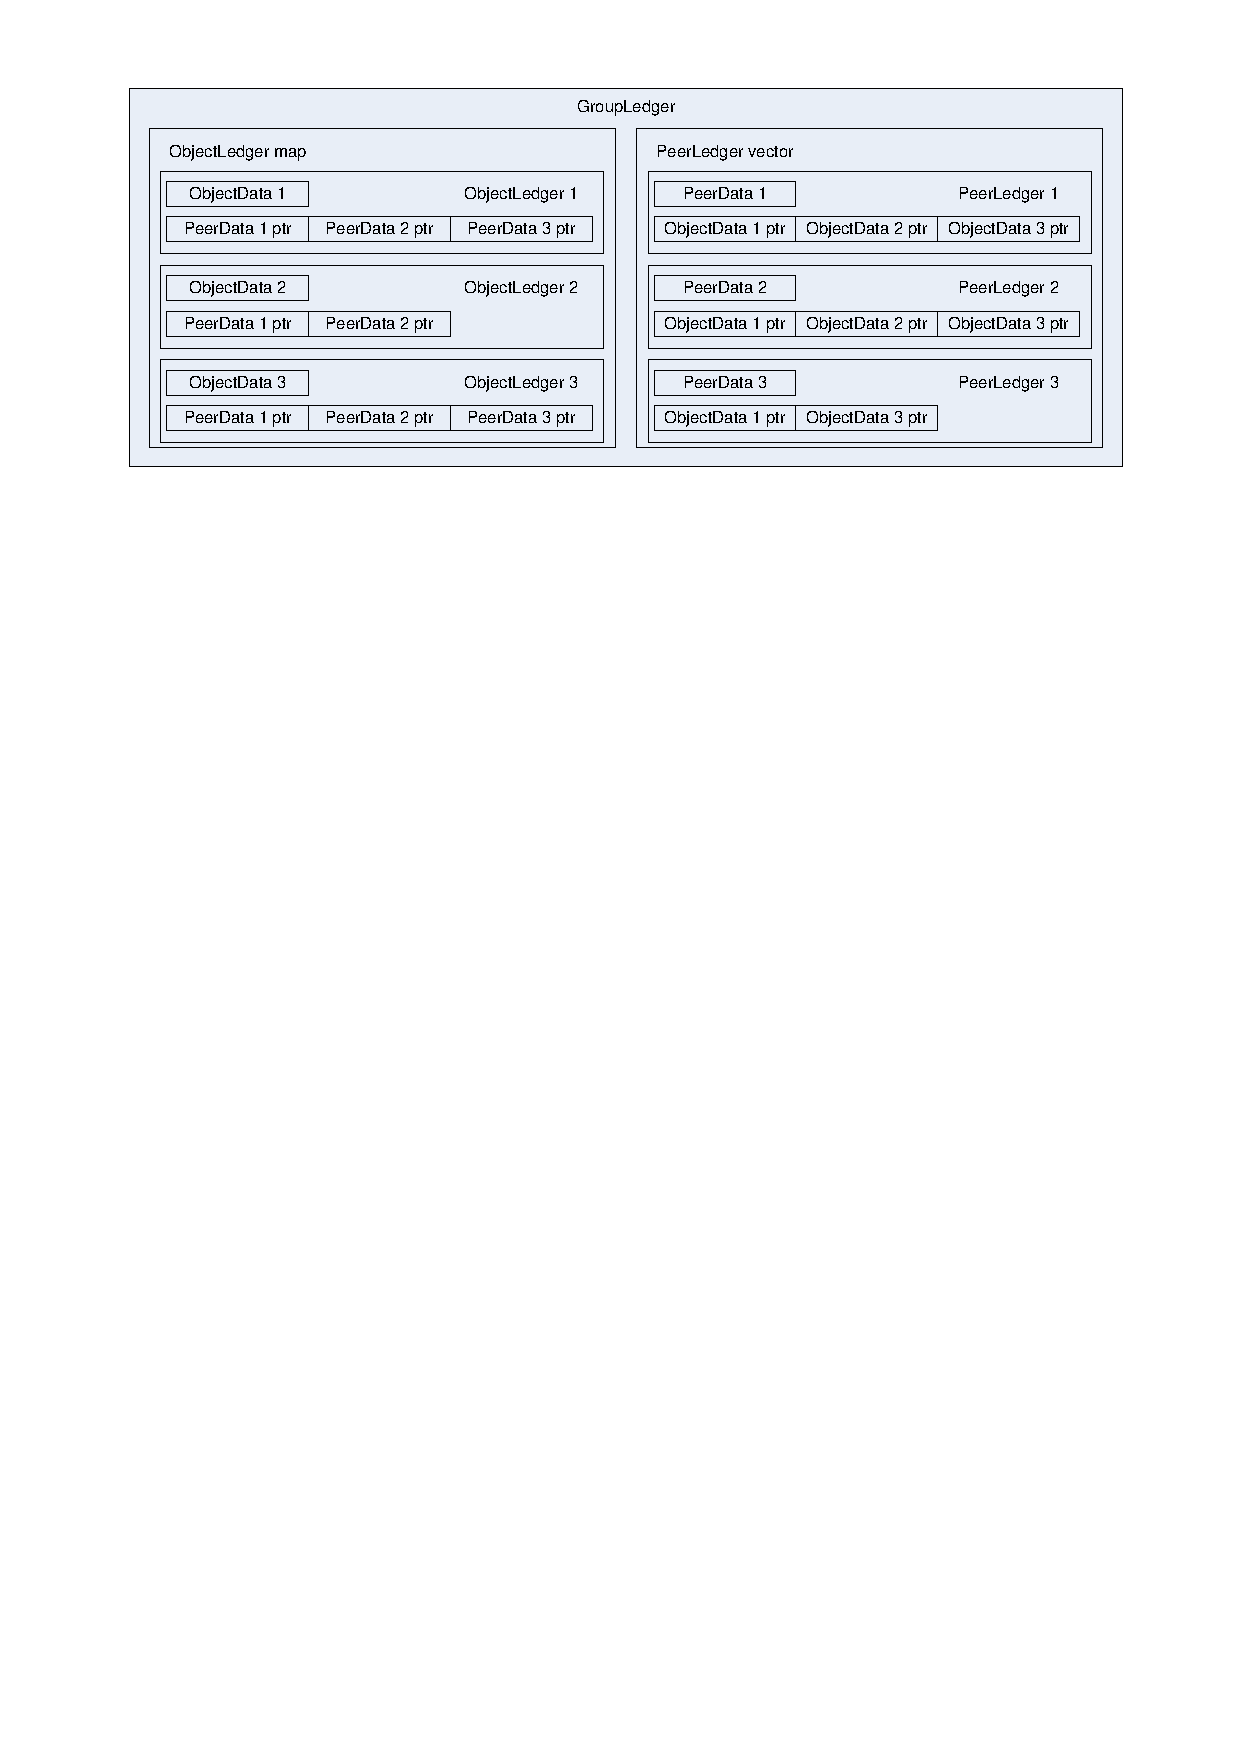
\includegraphics[clip=true, viewport=21mm 217mm 191mm 283mm, width=\columnwidth]{Group_ledger}
 \caption{Structure of the group ledger in the Pithos implementation.}
 \label{fig_group_ledger}
\end{figure}
%
Figure \ref{fig_group_ledger} shows the structure of the group ledger implementation. The group ledger is an abstract data type that maintains lists of all objects stored in the group, as well as all peers that are part of the group. The group ledger is used by peers and super peers to keep track of all group objects and peers.

The group ledger was designed for efficient storage, while still allowing high speed access to data. In order for the ledger to be efficient, it implements a map of object ledgers, where each object ledger contains object information and a list of peers where that object is stored on. The group ledger also contains a peer ledger list, where each peer ledger contains a list of objects that are housed on that peer.

In the object ledger, each entry in the peer list is a reference to peer information contained in the peer ledger. In the peer ledger, each entry in the object list is a reference to peer information contained in the object ledger. This means that peer and object information are only stored once, and always referred to by references. This dually linked structure allows for searching in any direction. Objects are stored in a map, since there might be thousands of objects in a group, compared to tens of peers. Efficient object lookup is, therefore, a priority, whereas sequential peer search is sufficient.

The ledger abstract data type is implemented using reference counting pointers (smart pointers), to avoid any memory leaks that might have occurred due to incorrect memory management of the large number of pointers present.

\subsection{Super peer node}
\label{pithos_module_types_sp_logic}

Since super peers are responsible for managing group membership and object repair, the super peer module requires its own super peer ledger to keep track of peers and objects in the group. The super peer logic sub-module implements all the required super peer mechanisms.

\subsubsection{Super peer logic}
The super peer logic module implements all the functionality of the super peer node, except for keeping track of group objects. The tasks of the super peer logic include:
\begin{itemize}
\item handling joining peers,
\item facilitating peer migration,
\item ensuring group consistency (Section \ref{group_consistency_implementation}),
\item initiating object repair, and
\item maintaining a list of group objects and a list of peers on which those objects are stored (Section \ref{pithos_module_types_ledgers}).
\end{itemize}

\subsubsection{Super peer ledger}

The super peer ledger is the same group ledger object used by all peers. The only difference is that it collects group-wide statistics on behalf of all group peers. This is possible, since the information of any group ledger in a specific group is the same.

\section{Implementation issues relating to key mechanisms}
\label{key_mechanisms}

%%%%%%%%%%%%%%%%%%%%%%%%%%%%%%%%%%%%%%%%%%%%%%%%%%%%%%%%%%%%%%%%%%%%%%%%%%
% For every mechanisms, reference where the results of that mechanism will
% be shown.
%%%%%%%%%%%%%%%%%%%%%%%%%%%%%%%%%%%%%%%%%%%%%%%%%%%%%%%%%%%%%%%%%%%%%%%%%%

While the previous chapter describes all key mechanisms, some adjustments had to be made to allow for correct functionality under Oversim. The key mechanisms that have simulation specific implementations are also discussed in this section.

\subsection{Joining the network and grouping}
\label{joining_and_grouping_imp}

It was decided that the work on Pithos would focus on improving the performance aspects of distributed storage systems, rather than on distributed joining and grouping mechanisms. It is accepted that this is work that has to be done, but it will be done as future research.

For the Pithos implementation, a single directory server was used. The directory server places joining peers into groups represented by super peers. The first task of a Pithos peer is to join the network and a group. This is done using the directory server, which possesses a static IP address and port that is known to every new peer and super peer.

\begin{figure}[htbp]
 \centering
 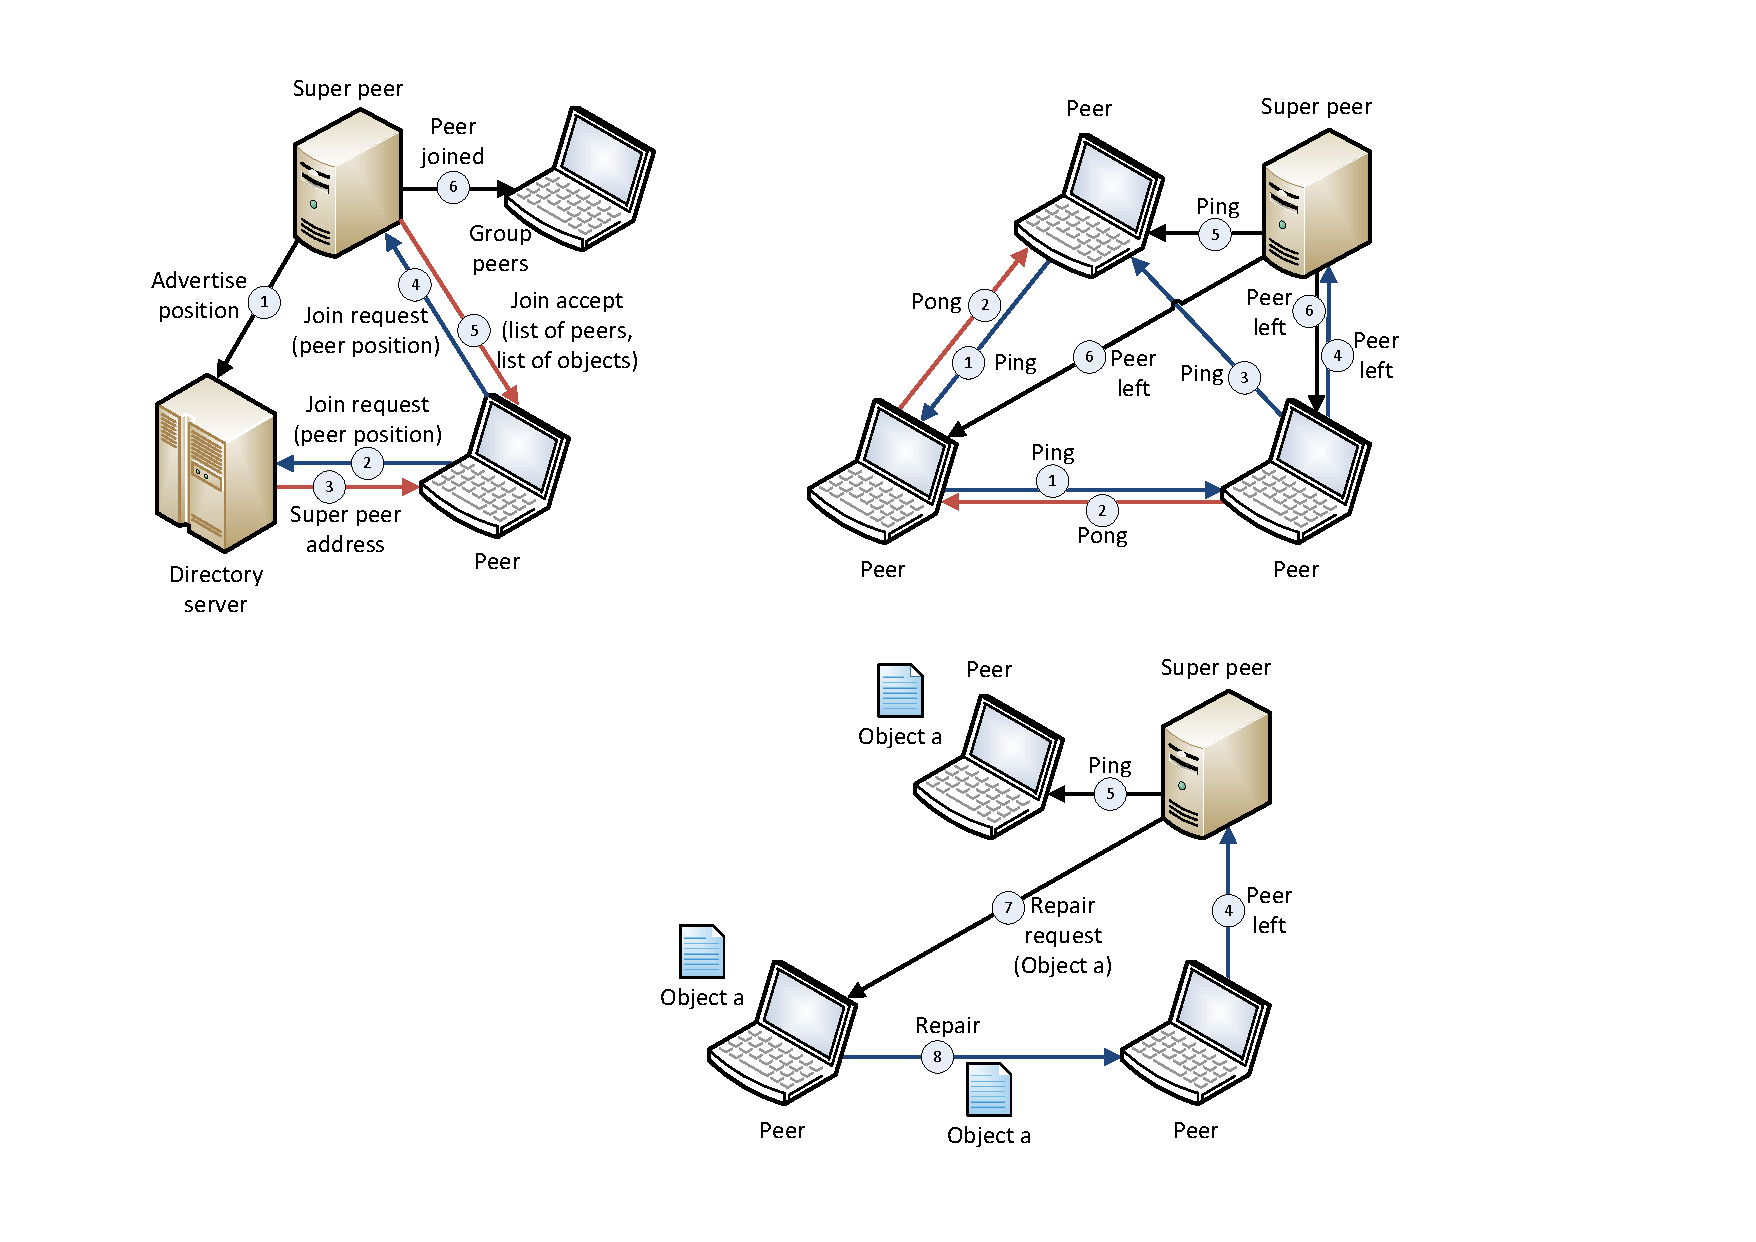
\includegraphics[clip=true, viewport=15mm 105mm 115mm 199mm, width=0.7\columnwidth]{Pithos_mechanisms}
 \caption{Pithos group join mechanism. The super peer publishes its VE location at the directory server, which allows the joining peer to be matched with a super peer and to join that super peer's group.}
 \label{fig_pithos_join}
\end{figure}
%
With reference to Figure \ref{fig_pithos_join}, the join and bootstrapping mechanism works as follows:
%
\begin{enumerate}
\item Whenever a super peer is created or potentially selected, it advertises its information with the directory server. This information includes its IP address, port and virtual location of the super peer in the VE.

\item When a peer wishes to join the network, it sends its current VE location to the directory server.

\item  The directory server then responds with the address of a super peer, representing an initial group which the peer can join.

\item The joining peer then sends the same type of join request to the supplied super peer address.

\item If the super peer accepts the joining peer, it sends that peer a list of all peers currently in the group, as well as a list of objects currently available in the group.

\item The super peer also informs all other group peers of the newly joined peer.
\end{enumerate}

The super peer can elect to accept or reject the joining peer. This extra step is intended to prevent groups from becoming overloaded. The super peer can supply an alternative address for the joining peer to contact. This extra step is also intended to compensate for the movement of super peers. If a super peer moves, and by the time a joining peer contacts a super peer there is another super peer in closer range, the super peer receiving the join request can supply the joining peer with the address of the closer super peer.

Because Pithos is not functioning in an actual VE, peers have no locations. For simulation purposes, each super peer is assigned a random location created by sampling both an x and a y coordinate from a uniform random distribution in a fixed range (0 to 100). Joining peers are assigned positions in the same uniform random manner when they are initialised.

These positions are used by the super peers and peers when contacting the directory server. The directory server supplies the peer with the address of the closest super peer to join. This is an implementation of a simple centralised grouping algorithm. Super peers effectively control certain areas in the VE, based on their and their neighbours' locations.

Although the distributed grouping techniques discussed in Section \ref{grouping_design} are exchanged for a simple centralised scheme, it serves its purpose to group all peers into groups controlled by super peers for the simulation. In a practical implementation, this solution is still applicable, but the directory server might become overloaded. The distributed grouping and joining mechanism is, therefore, recommended.

\subsection{Group migration}
\label{group_migration_implementation}

To simulate the effect that user movement will have on objects stored in Pithos, PithosTestApp is designed to generate position updates.

PithosTestApp simulates a user moving around in a virtual world. This is done by having PithosTestApp generate a new random position chosen in the same way as when a node joined a group: by selected x and y coordinates in a uniformly random fashion. A position update timer determines when a node's position should change. When a new position is generated by PithosTestApp, this is sent to the group storage module, which then initiates the group migration mechanism.

As avatars move around in the virtual world and PithosTestApp sends position updates to Pithos, Pithos queries the directory server at regular intervals with new avatar positions, using the same mechanism described for joining a group in Section \ref{joining_and_grouping_imp}. Directory server query intervals are long enough to prevent overloading of the directory server, but short enough to ensure peers have an up-to-date view of the group. The peer then receives a new super peer address from the directory server, if this address is different from the address of the currently known super peer. When a new address is received, Pithos initiates group migration.

It is accepted that the movement scheme does not match the way users move in a virtual world. Modelling accurate user movement is, however, not considered important for the current Pithos simulation. Storing and retrieving objects in Pithos only depends on which group a user occupies, the group density and how Pithos handles a user that moves to another group. The order in which a user might enter groups or, in fact, the specific group that a user moves to, is not considered important. All that is important is how objects are handled when any group migration occurs and how group density affect the performance.

The effect of user movement traces on the performance of Pithos will be explored as future research.

\subsection{Tracking requests}
\label{pending_rpcs_implementation}

When sending a request to a destination peer, the destination peer might leave the group before it can receive the request or respond to it. No response will, therefore, be sent to the source peer, which might cause some requests to remain unresolved. For example, if safe storage is used and the system waits for all responses before informing the higher layer of the request status, the higher layer will never be informed if a destination node has left. A mechanism is required to handle nodes leaving the group.

The solution is for the super peer logic, peer logic and DHT modules to track all requests sent, and link every outstanding request with a timeout. Every one of those modules contains a pending requests list. Each pending request is uniquely identified by the RPC ID received from PithosTestApp, which uniquely identifies a specific request. Each pending request from the higher layer usually generates multiple messages to DHT storage, and multiple nodes in the group via group storage.

Every request sent out by the DHT storage or group storage modules contain the RPC ID of the original request from PithosTestApp. The RPC ID is copied into the response at the destination location. This allows every response to be linked to the original request that generated it. When a response is received from a peer, the pending request for the RPC ID for that peer is removed from the pending requests list.

Every pending request is also linked to a timeout. If the timeout expires, the pending request is removed and a failure response is generated and sent to the higher layer. This mechanisms ensures that all requests will always receive all expected responses. The timeout are the same timeouts use to detect whether a peer has left the group, as discussed in Section \ref{leave_design}.

It is accepted that this mechanism may cause false negatives if there is a delay due to congestion in the network. This situation can be avoided by making the timeout sufficiently long, as will be shown in Section \ref{group_storage_eval}.

\subsection{Quorum}
\label{object_verification_implementation}

To test the quorum mechanism, the idea of malicious nodes was added to Pithos. When a node starts, there is some percentage change that it will be designated as a malicious node. Whenever a malicious node receives a retrieve request, it retrieves the requested object, but alters it in some random way. This altered object is then sent to the requesting peer. A flag saying that the object has been altered is also sent, for statistics gathering.

The reliability of Pithos could be investigated for various levels of malicious nodes in the network, as discussed in Section \ref{malicious_results}.

\subsection{Group consistency}
\label{group_consistency_implementation}

With peers constantly joining and leaving the network and transferring between groups, an issue that arises is group consistency. It is important that all peers within a group share the same view of that group. If this is not the case, some peers might never be chosen to store data and this will decrease the fairness in the system. Another reason is that for the sake of scalability, peers do not service requests from peers outside of their groups. Group inconsistencies might also lead to nodes becoming isolated from any group, which basically disconnects that node from the P2P network. A primary source of inconsistencies was the fact that it takes time to inform all group peers of a peer that left and that it takes time to inform all group peers of a peer that joined.

To ensure group consistency, the following improvements were made to Pithos:
%
\begin{enumerate}
\item The super peer stores the information of the last peer that left and the last peer that joined.
\item Peers store information of the last peer that left.
\item Every time a new peer joins, the super peer informs the joining peer of the last peer that left.
\item Every peer ignores messages from the last peer that left.
\item Timeouts are adjusted as a function of available network bandwidth.
\item Group identification information was added to every request, identifying the group where a messages originates from.
\item If a peer received a response from a peer situated in another group, the peer making the request removes the information of the peer that responded to the request from its group ledger.
\end{enumerate}

For a detailed discussion on group consistency and the reasons for the various solutions, the reader is referred to Appendix \ref{chp:GROUP_INCONSISTENCY}. The appendix is, however, not required for an understanding of the rest of this work.

\begin{figure}[htbp]
 \centering
 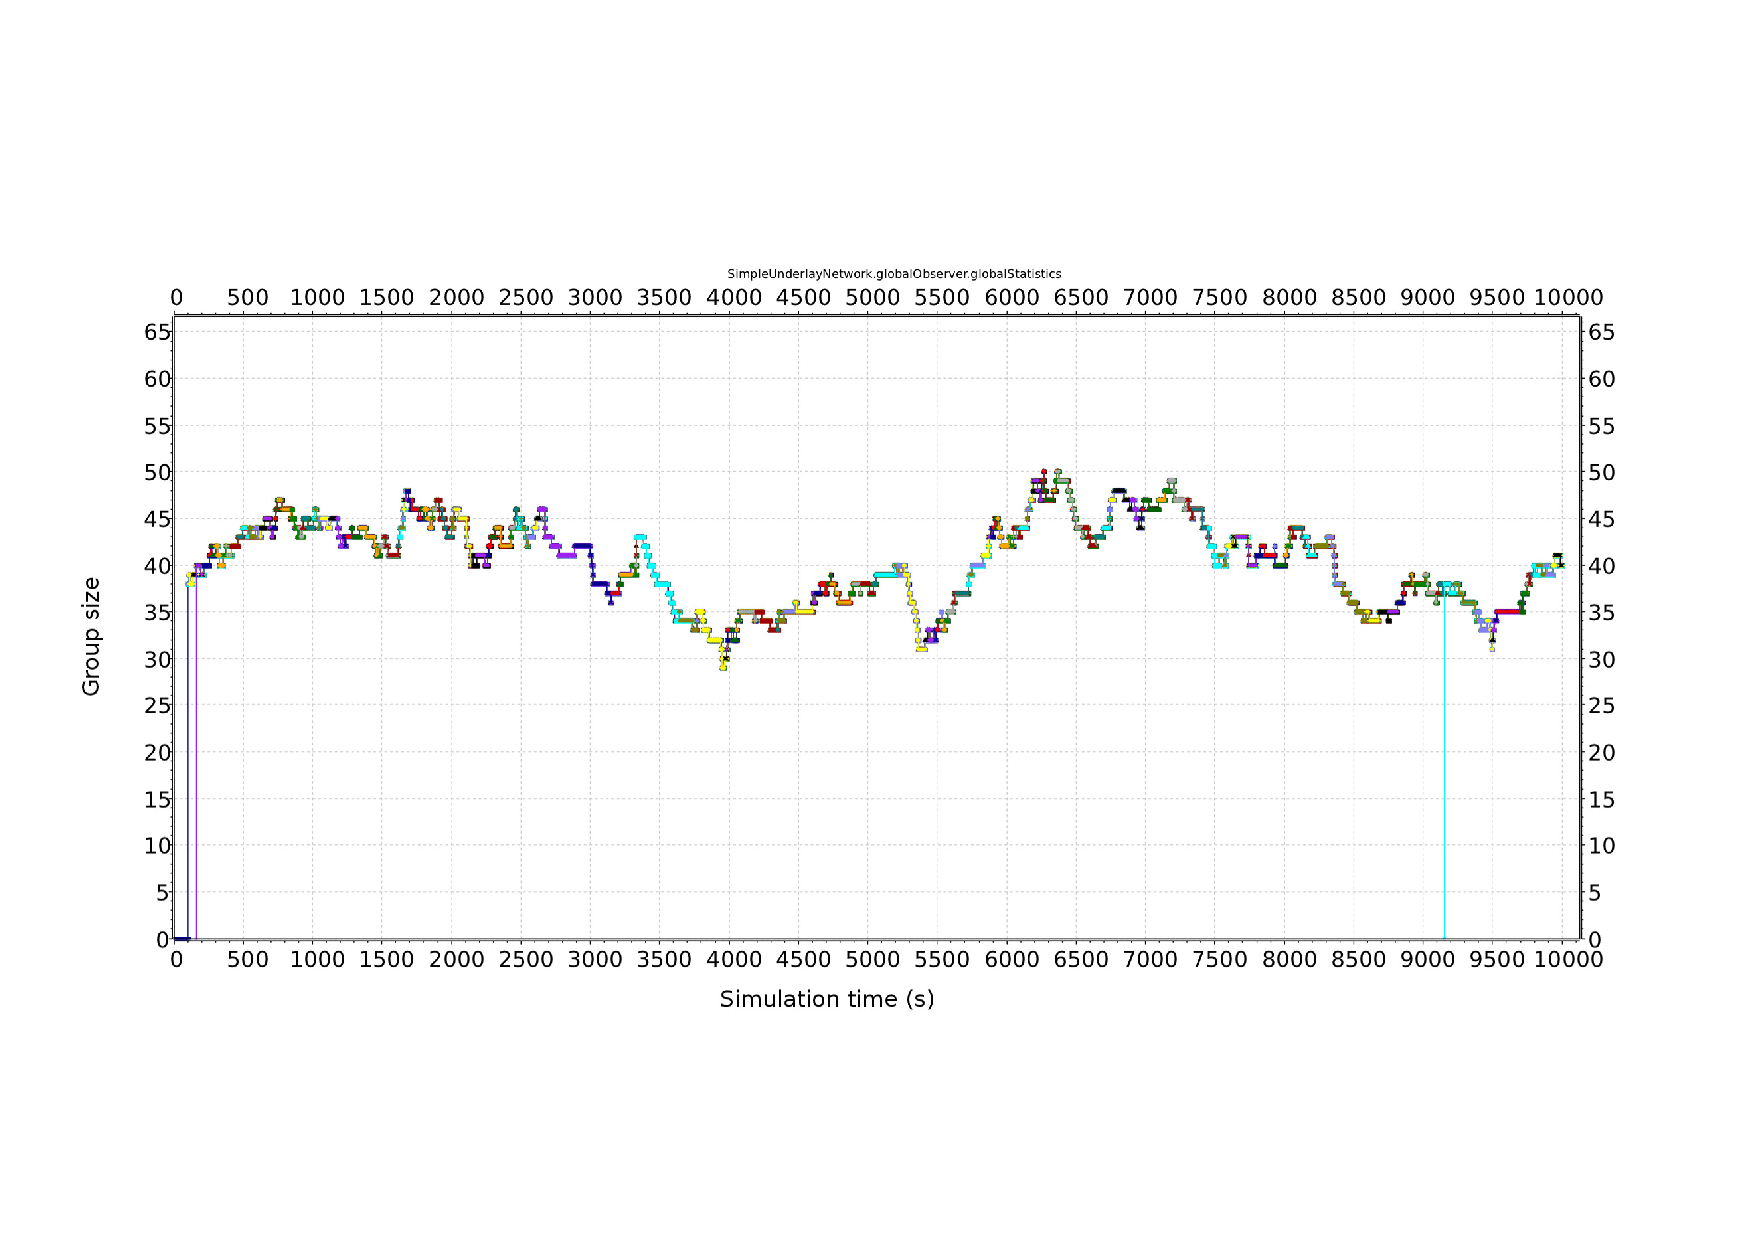
\includegraphics[clip=true, viewport=12mm 35mm 275mm 165mm, width=\columnwidth]{gc_final_png}
 \caption{Group consistency after all improvements}
 \label{fig_gc_final}
\end{figure}
%
Figure \ref{fig_gc_final} shows the view of group containing 40 peers on average as a function of time. Every peer reports its view of the group size at 1s intervals and those views are overlayed and plotted.

To calculate group consistency, each vector was compared with the super peer's view of the group. For each of the 251 nodes that joined and left the group over the 10,000s simulation time, error vectors were calculated by calculating the difference between the super peer group size vector and the group size vector of every other peer in the group for the duration that a peer was part of the group.

The mean and standard deviations were then calculated for each of these vectors to form two new mean error and standard deviation error vectors. The mean and standard deviation of the mean error vector is 0.0096 and 0.0104 respectively. The mean and standard deviation of the standard deviation vector is 0.0941 and 0.1338.

This data shows that on average there is a 0.0096 peer difference between the number of peers that the super per perceives and the number of peers that the rest of the group peers perceive within every 1s interval. This is considered a sufficiently high level of consistency for the purpose of the Pithos evaluation.

\section{PithosTestApp implementation}
\label{pithostestapp}

Some application was required that would generate requests for Pithos and collect statistics on how well Pithos services those request. The application that was implemented to perform this duty is PithosTestApp.

PithosTestApp is located one layer above Pithos in the generic consistency architecture, called the object updater. It should be noted that PithosTestApp has no purpose other than to test Pithos. It is therefore supposed to present an aggregation of all the higher layer modules to Pithos.

PithosTestApp has four functions:
\begin{enumerate}
\item Generate store, retrieve and modify requests.
\item Correctly handle all responses received form Pithos.
\item Generate position updates.
\item Collect statistics to determine how successfully Pithos handles the requests.
\end{enumerate}

\subsection{Store requests}

PithosTestApp periodically generates store requests of random sizes. The sizes of these requests are based on the literature on how large game objects usually are. This includes an evaluation that was performed on the size of game objects in Ultima Online and the measurements acquired from the Donnybrook architecture \cite{Bharambe_Donnybrook}.

All store requests are sent to Pithos in the lower layer. When a response is received that an object has been successfully stored, the object information is added to a global map, containing all generated objects.

\subsection{Retrieve requests}

The global object map is not available to Pithos and is only used by PithosTestApp to enable object retrieval and for retrieved objects to be verified. Objects in the global object map are grouped by the group they are stored in.

PithosTestApp periodically generates retrieve requests for random objects. An object is selected from the global object map and a request for this object is made to Pithos. The object itself is never supplied to Pithos, other than when it is stored.

PithosTestApp can generate in-group object requests with a given probability. This is to test how well Pithos will function when distance-based storage is implemented to store objects. The assumption is that, with distance-based storage, a high number of retrieval requests will be for nodes within the same group, as opposed to out-of-group nodes.

When a response is received, statistics are recorded on whether the request was a success or failure as well as the reason. If the retrieval is a success, the returned object is compared with the object in the global object store to determine whether the retrieved object's contents physically matches the object contents in the global object store. Verification is mostly used when malicious peers exist and there is a chance that Pithos might send the information of a corrupted object to the higher layer.

\subsection{Modify requests}

PithosTestApp periodically generates modify requests. It selects a random object from the global object map, selects a random variable of that object to modify and assigns a new random value to that parameter. The new parameter value is then encapsulated in a modify request sent to Pithos.

\subsection{Position updates}

When group migration is enabled, PithosTestApp generates regular position updates to allow Pithos to test group migration.

\section{Conclusion}

An overview of the Oversim simulation framework was presented and it was also explained how Oversim was extended to support the generic consistency architecture. Some implementation issues encountered during the Pithos implementation were also discussed. The main purpose of this chapter is to link the conceptual design with the Oversim simulation implementation of Pithos; to provide concrete explanations on how some of the key mechanisms were implemented.
